\documentclass[11pt]{article}

% ─── Packages ─────────────────────────────────────────────────────
\usepackage[margin=1in]{geometry}
\usepackage{graphicx}
\usepackage{amsmath, amssymb}
\usepackage{booktabs}
\usepackage{hyperref}
\usepackage{xcolor}
\usepackage{enumitem}
\usepackage{caption}
\usepackage{subcaption}
\usepackage{float}
\usepackage{array}
\usepackage[numbers]{natbib}
\usepackage{tikz}
\usepackage{fancyhdr}
\usepackage{titlesec}
\usepackage{multirow}

\usetikzlibrary{arrows.meta, positioning, shapes.geometric, fit}

\graphicspath{{report_assets/report_assets/}{experiment_assets/training_curves/}{experiment_assets/confusion_matrices/}}

\hypersetup{colorlinks=true, linkcolor=blue!60!black, citecolor=green!50!black, urlcolor=blue!70!black}

% ─── Header and Footer ─────────────────────────────────────────────
\pagestyle{fancy}
\fancyhf{}
\rfoot{\thepage}
\renewcommand{\headrulewidth}{0pt}

% ─── Title Formatting ─────────────────────────────────────────────
\title{\textbf{Classification of Indian Lepidoptera Species}\\
\Large Fine-Grained Butterfly Recognition Under Domain Shift}

\author{
  Akshit Bansal, Kriti Chaturvedi
}

\date{}

% ─── Section Formatting ─────────────────────────────────────────────
% \titleformat{\section}
%   {\normalfont\large\bfseries}
%   {}
%   {0em}
%   {}

% \titleformat{\subsection}
%   {\normalfont\normalsize\bfseries}
%   {}
%   {0em}
%   {}

\setlength{\parskip}{0.5em}
\setlength{\parindent}{0em}
\emergencystretch=1em

\begin{document}
\maketitle

\section{Abstract}
Fine-grained classification of Indian Lepidoptera species presents compounding challenges: spatial information collapse in channel attention, progressive texture-cue loss through pooling, and extreme long-tail class imbalance. We present IndoLepAtlas, a curated 60,641-image, 966-species India-specific butterfly dataset with geotemporal metadata, early life-stage documentation, and 703 images of 127 larval host plant species. We conduct a systematic evaluation spanning six architectures--ResNet-101, EfficientNet-B5, ViT-B/16, and our ConvNeXt-S variants with Coordinate Attention (CA), Multi-Level Feature Interaction (MLFI), and geotemporal fusion--alongside an 11-configuration ablation across loss dynamics, feature fusion, and transfer-learning strategies. Our geotemporal model achieves \textbf{89.38\% Top-1 accuracy} and \textbf{98.01\% Top-5} with 2.1$\times$ fewer parameters than ViT-B/16 (89.99\% Top-1), while achieving the best sparse-class accuracy (87.43\%) across all models. A geo-shuffled control confirms the geotemporal branch learns genuine biogeographic priors ($-$3.02\% Top-1 on ablation). Cross-referencing against iNaturalist reveals 69.3\% of our species have fewer than 100 India-specific records, establishing IndoLepAtlas as a critical resource for India-focused Lepidoptera research.

\section{Introduction and Motivation}

India's 1,500+ Lepidoptera species represent one of the world's richest butterfly biodiversity hotspots. Automated classification from field photographs is critical for ecological monitoring and conservation planning. Yet this task fundamentally differs from standard benchmarks: discriminative features are spatially precise (eyespot location separates genera), hierarchically distributed across scales (texture bands vs overall wing morphology), and unevenly sampled (dominant species exceed 500 images while 400 rare species have $<$50 images).

Existing global biodiversity datasets--iNaturalist~\cite{vanhorn2018inaturalist}, GBIF--dilute India-specific subspecies representation. Many Indian endemic and regionally restricted species have fewer than 100 research-grade observations in global repositories, creating a critical data gap for conservation-focused AI systems. Furthermore, no existing butterfly classification dataset integrates geotemporal metadata (biogeographic zone, observation season) or documents larval host plant associations--ecological dimensions that could substantially improve classification accuracy and enable applications beyond species identification, such as early-stage detection and habitat suitability mapping.

Standard CNNs fail on this task in predictable ways. Channel attention mechanisms like SE-Net~\cite{hu2018squeeze} collapse spatial dimensions through global average pooling, discarding the positional information essential for wing pattern discrimination. Deep pooling progressively destroys fine-grained texture cues, routing only high-level semantics to the classifier. Uniform sampling over-indexes on common species, starving rare classes of gradient signal.

We make the following contributions:
\begin{enumerate}[label=(\arabic*)]
    \item \textbf{IndoLepAtlas dataset:} A curated 60,641-image, 966-species India-specific Lepidoptera dataset with GPS coordinates, observation dates, 9-zone biogeographic mapping, early life-stage documentation and 703 images of 127 larval host plant species--the first butterfly dataset to integrate ecological metadata at this scale.
    \item \textbf{Systematic baseline establishment:} An 11-configuration ablation study across loss dynamics, architectural feature fusion, and transfer-learning strategies, plus a 6-model comparison (ResNet-101, EfficientNet-B5, ViT-B/16, MLFI Warmup, Geo-Shuffled control, Geotemporal), providing reproducible baselines for future work on IndoLepAtlas.
    \item \textbf{Domain-shift analysis:} Empirical demonstration that ImageNet features are fundamentally misaligned with entomological morphology, with head-only probing achieving just 53.20\% and exhibiting a striking Dense/Sparse accuracy inversion.
    \item \textbf{Geotemporal fusion:} First integration of biogeographic zone and seasonal embeddings into a butterfly classification pipeline, achieving 89.38\% Top-1 with 2.1$\times$ fewer parameters than ViT-B/16, and verified via geo-shuffled ablation.
\end{enumerate}

\section{Related Work}

\subsection{Fine-Grained Visual Classification}
Fine-grained visual classification (FGVC) aims to distinguish subordinate categories within a superclass--bird species~\cite{wah2011cub}, dog breeds, car models. Key benchmarks include CUB-200-2011~\cite{wah2011cub} (200 bird species, 11,788 images) and iNaturalist~\cite{vanhorn2018inaturalist} (5,000+ species, 675,000 images). Architecturally, the field has progressed from bilinear pooling through channel attention (SE-Net~\cite{hu2018squeeze}) to multi-level feature fusion (FGBNet~\cite{yuan2025fgbnet}). Vision Transformers~\cite{dosovitski2021image} achieve strong results on large-scale FGVC but require substantial data. Coordinate Attention~\cite{hou2021coordinate} offers a lightweight alternative that preserves spatial structure--a property we exploit for wing-pattern localisation.

\subsection{Insect and Butterfly Classification}
Automated insect classification has gained momentum with datasets for crop pests~\cite{amarathunga2022thrips}, thrips, and general entomology. For Lepidoptera specifically, existing systems rely on standard transfer learning from ImageNet without addressing the domain gap. Amarathunga et al.~(2021) identify temporal distribution, geographic context, and life-stage variation as open problems in insect classification--problems that IndoLepAtlas directly addresses through its metadata design. No prior work integrates geotemporal features into an end-to-end butterfly classification pipeline.

\subsection{Geotemporal Features in Ecological ML}
Species distribution modelling (MaxEnt, random forests on bioclimatic variables) has long used geographic and seasonal features for predicting species occurrence. iNaturalist's geo-aware species suggestions demonstrate the practical value of location priors. However, these approaches operate as separate prediction systems rather than fusing geotemporal context into the visual classification pipeline itself. Our geotemporal fusion module bridges this gap by concatenating learned biogeographic zone embeddings and cyclic seasonal encodings with visual features before classification.

\section{IndoLepAtlas Dataset}

\subsection{Collection and Curation}
IndoLepAtlas comprises 61,344 images spanning 970 butterfly species and 139 larval host plant species, curated from the Indian Lepidoptera web atlas and iNaturalist with rigorous quality control. The filtering pipeline removes non-butterfly entries, resolves taxonomic synonyms, and separates early life-stage images (9,804) from adult specimens (50,686) using both metadata tags and filename pattern matching. Adult images are used for classification training; early-stage images are retained as labelled auxiliary data for future life-stage detection and species-lifecycle modelling.

\subsection{Taxonomic and Geographic Coverage}
The dataset covers six butterfly families: Nymphalidae (18,054), Lycaenidae (16,985), Hesperiidae (12,361), Pieridae (6,132), Papilionidae (5,826), and Riodinidae (1,132)--representing approximately 64\% of India's known butterfly diversity. Geographic coverage spans 36 Indian states and territories mapped to 9 biogeographic zones, with primary contributions from Maharashtra (10,198), Karnataka (8,121), and Kerala (6,795). Metadata coverage: 99.8\% location, 76.2\% date, 64.8\% sex missing (acknowledged limitation). Temporal distribution spans all 12 months with a monsoon peak (August--November; September: 5,198, October: 7,228), reflecting natural butterfly activity patterns.

\subsection{Unique Features: Early Stages and Host Plants}
Unlike existing FGVC datasets, IndoLepAtlas documents the ecological context of each species:
\begin{itemize}[nosep]
    \item \textbf{Early life-stage images} Labelled caterpillar/pupa/egg photographs enable future work on life-stage classification and conservation efforts by early species prediction/detection, as well as early pest detection--critical for agricultural monitoring where caterpillar identification precedes adult emergence by weeks.
    \item \textbf{Larval host plant associations} (127 plant species with 703 images) document butterfly--plant ecological dependencies. This data supports habitat suitability modelling: a species cannot persist where its host plant is absent, providing a strong ecological prior for distribution prediction.
    \item \textbf{Geotemporal metadata} (GPS $\to$ 9 biogeographic zones, observation dates $\to$ cyclic month encoding) enables fusion of ecological context into visual classification.
\end{itemize}

\subsection{Class Distribution and Evaluation Protocol}
Class distribution ranges from 203 images (\emph{Papilio protenor}) to $<$5 images (tail species). Classes are stratified into \textbf{Dense} ($\geq$50 images, 339 classes) and \textbf{Sparse} ($<$50 images, 627 classes) strata. Data is split into train (79.3\%, 48,630), validation (9.2\%, 5,649), and test (11.5\%, 7,065) partitions.

\subsection{Coverage Gap Analysis}
Cross-referencing IndoLepAtlas species against iNaturalist India research-grade observations (961 species queried via the iNaturalist API) reveals that 69.3\% of our species have fewer than 100 India-specific iNat records, and 145 species (15.1\%) have zero records. This confirms that global repositories severely under-represent India-specific Lepidoptera diversity, establishing IndoLepAtlas as a critical complementary resource.

\begin{table}[H]
\centering
\caption{IndoLepAtlas species representation in iNaturalist India.}
\label{tab:inat_coverage}
\small
\begin{tabular}{@{}lcc@{}}
\toprule
\textbf{iNat India Records} & \textbf{\# Species} & \textbf{\% of Dataset} \\
\midrule
0 (absent)      & 145 & 15.1\% \\
1--10           & 249 & 25.9\% \\
11--50          & 194 & 20.2\% \\
51--100         & 78 & 8.1\% \\
101--500        & 147 & 15.3\% \\
$>$500          & 148 & 15.4\% \\
\bottomrule
\end{tabular}
\end{table}

% === Cross-Dataset Comparison Table ===
\begin{table}[H]
\centering
\caption{Comparison with existing fine-grained classification datasets.}
\label{tab:dataset_comparison}
\small
\begin{tabular}{@{}lccccc@{}}
\toprule
\textbf{Dataset} & \textbf{Species} & \textbf{Images} & \textbf{Geo} & \textbf{Temporal} & \textbf{Host Plants} \\
\midrule
CUB-200-2011~\cite{wah2011cub}    & 200   & 11,788  & \texttimes & \texttimes & \texttimes \\
iNaturalist~\cite{vanhorn2018inaturalist} & 5,089 & 675,170 & \checkmark & \checkmark & \texttimes \\
IP102               & 102   & 75,222  & \texttimes & \texttimes & \texttimes \\
\textbf{IndoLepAtlas} & \textbf{966} & \textbf{60,641} & \checkmark & \checkmark & \checkmark \\
\bottomrule
\end{tabular}
\end{table}

\section{Experimental Setup}

We execute experiments on a DGX V100 cluster in two phases. First, a systematic 11-configuration ablation across three experimental units: Unit~I (loss dynamics, 30 epochs), Units~II and III (architecture and freezing, 40 epochs). All ablation experiments use a ConvNeXt-Tiny backbone~\cite{liu2022convnext} with AdamW optimisation (differential learning rates: backbone $0.1\times$, new heads $10^{-4}$), cosine annealing with 5-epoch warmup, mixed precision AMP, and macro-F1 checkpoint selection to ensure long-tail sensitivity.

Second, a 6-model comparison study (40 epochs each) evaluating ResNet-101 (44.5M params), EfficientNet-B5 (30.3M), ViT-B/16 (86.5M), MLFI Warmup (ConvNeXt-S + CA + MLFI, 40.8M), and our geotemporal model (ConvNeXt-S + CA + MLFI + Geo, 40.8M) with a geo-shuffled control. All comparison models use CE loss, AdamW ($lr=10^{-4}$), and balanced sampling. Dataset split: 40,260 train / 4,673 val / 5,865 test images across 966 species.

\section{Core Findings}

\subsection{Unit I: Long-Tail Loss Dynamics (30 Epochs)}

\textbf{Question:} \emph{How do different loss formulations and sampling strategies impact representational capacity on long-tailed fine-grained distributions?}

We test cross-entropy (CE) and Focal Loss~\cite{lin2017focal} across balanced and unbalanced sampling. Results are summarised in Table~\ref{tab:master} (Unit~I rows).

\begin{figure}[H]
\centering
\includegraphics[width=0.95\linewidth]{report_assets/report_assets/plots/unit1_training_curves.png}
\caption{Unit~I training curves: validation loss and accuracy over 30 epochs for all four loss--sampling configurations.}
\label{fig:unit1_curves}
\end{figure}

\begin{figure}[H]
\centering
\includegraphics[width=0.65\linewidth]{report_assets/report_assets/plots/unit1_bar_comparison.png}
\caption{Unit~I metric comparison: Top-1 accuracy, Macro-F1, Dense and Sparse accuracy across loss--sampling strategies.}
\label{fig:unit1_bars}
\end{figure}

\textbf{The ``Unbalanced'' illusion.} CE~+~Unbalanced achieves the highest raw Top-1 accuracy (87.60\%), but this masks severe stratum imbalance: Dense accuracy inflates to 91.22\% while Sparse accuracy drops to 80.35\%. The macro-F1 plummets to 80.23\%--a 5.25-point gap below the balanced variant--confirming the model abandons rare species to maximise majority-class performance.

\textbf{CE + Balanced as optimal compromise.} Balanced sampling forces equitable gradient allocation, compressing the Dense--Sparse gap to just 1.83 points (87.67\% vs 85.84\%) while achieving the highest macro-F1 (85.48\%) and macro-precision (87.43\%). The mechanism is direct: inverse-frequency sampling ensures rare-class gradients remain proportional regardless of natural distribution skew.

\textbf{The Focal Loss penalty.} Focal Loss~\cite{lin2017focal} with $\gamma=2$ achieves the highest Sparse-class accuracy (86.40\% under balanced sampling) but severely degrades Dense-class performance to 80.85\%. In 966-class fine-grained settings, the $(1-p_t)^\gamma$ modulation over-penalises well-classified easy examples (typically Dense strata), damaging foundational feature extraction for common species. Focal~+~Unbalanced partially recovers Dense accuracy (85.70\%) but at the cost of Sparse performance. This contradicts the assumption that loss-function sophistication universally solves long-tail problems--explicit sampling proves more reliable.

\subsection{Unit II: Feature-Fusion Ablation (40 Epochs)}

\textbf{Question:} \emph{Where is the optimal structural transition point for integrating attention mechanisms, and does multi-level feature integration improve fine-grained classification?}

We ablate structural complexity across three progressive phases (Table~\ref{tab:master}, Unit~II rows).

\begin{figure}[H]
\centering
\includegraphics[width=0.95\linewidth]{report_assets/report_assets/plots/unit2_training_curves.png}
\caption{Unit~II training curves: validation loss and accuracy over 40 epochs for Baseline, +CA, and +CA+MLFI architectures.}
\label{fig:unit2_curves}
\end{figure}

\begin{figure}[H]
\centering
\includegraphics[width=0.65\linewidth]{report_assets/report_assets/plots/unit2_bar_comparison.png}
\caption{Unit~II metric comparison: progressive feature-fusion architecture performance.}
\label{fig:unit2_bars}
\end{figure}

\textbf{Coordinate Attention preserves spatial morphology.} Introducing Coordinate Attention~\cite{hou2021coordinate} after each backbone stage (Phase~2) yields the best overall configuration: 86.77\% Top-1, 85.75\% macro-F1, and a notable 1.29-point improvement in Sparse-class accuracy (86.76\% $\to$ 88.05\%). CA decomposes channel-spatial attention into two 1D processes: $\mathbf{z}_h = \text{AvgPool}_W(\mathbf{X})$ and $\mathbf{z}_w = \text{AvgPool}_H(\mathbf{X})$, preserving directional structure naturally suited to butterfly morphology (horizontal banding, vertical vein streaking). Unlike SE-Net's global average pooling, CA retains \emph{where} a pattern occurs--critical when eyespot position on forewing vs hindwing separates genera. The overhead is minimal ($<$0.5\% added parameters), making CA a high-value, low-cost intervention.

\textbf{MLFI: powerful but over-parameterised.} Phase~3 concatenates features from all four backbone stages (192 + 384 + 96 + 768 = 1,440 dimensions)~\cite{yuan2025fgbnet} to preserve texture cues destroyed by successive pooling. This adds approximately 12M parameters. At 40 epochs, MLFI reaches 84.43\% Top-1 and 86.66\% Sparse accuracy--demonstrating that multi-level fusion does benefit rare classes--but creates a 2.07-point Top-1 gap versus the baseline. The newly initialised MLFI fusion layers (Xavier initialisation, full learning rate) create an optimisation imbalance with the near-converged backbone ($0.1\times$ learning rate), resulting in a poorly conditioned loss landscape. Because early layers capture high-frequency textural variance that varies fiercely under different lighting, forcing these raw activations into the classification head introduces feature noise that overwhelms the refined late-layer semantic signals.

\subsection{Unit III: Transfer Learning Layer Freezing (40 Epochs)}

\textbf{Question:} \emph{Which hierarchical layers contain domain-agnostic representations versus domain-specific concepts, and what is the optimal adaptation pathway for non-standard image domains?}

\begin{figure}[H]
\centering
\includegraphics[width=0.95\linewidth]{report_assets/report_assets/plots/unit3_training_curves.png}
\caption{Unit~III training curves: validation loss and accuracy over 40 epochs for all four layer-freezing strategies.}
\label{fig:unit3_curves}
\end{figure}

\begin{figure}[H]
\centering
\includegraphics[width=0.65\linewidth]{report_assets/report_assets/plots/unit3_bar_comparison.png}
\caption{Unit~III metric comparison: layer-freezing strategy performance (see Table~\ref{tab:master}, Unit~III rows).}
\label{fig:unit3_bars}
\end{figure}

\textbf{The domain-shift wall.} Head-only linear probing--freezing the entire backbone and training only a classification head--achieves just 53.20\% Top-1 on 966 species. Dense-class accuracy collapses to 44.46\%, worse than Sparse-class accuracy (70.75\%), a striking inversion that reveals ImageNet features are not merely \emph{incomplete} but actively \emph{misaligned} with Lepidoptera morphology. SE-Net activations encode ``furry surface textures'' and ``rounded shapes,'' not ``submarginal band'' or ``discal spot.'' Fine-grained biological classification is fundamentally a domain-shift problem~\cite{dosovitski2021image} disguised as a classification problem.

\textbf{Early vs late block freezing.} Freezing late blocks (84.33\%) slightly outperforms freezing early blocks (83.77\%). This implies that the early-layer Gabor-like edge detectors require significant recalibration to adapt to butterfly wing scales, biological venation, and field photography conditions. Adapting early layers creates a stronger foundation for the frozen late layers to build upon. The inter-strategy variance is small ($\Delta < 1\%$), indicating that under sufficient training budget, any partial-freezing strategy approaches end-to-end performance.

\textbf{End-to-end supremacy.} Full gradient backpropagation achieves the best macro-F1 (84.11\%) and the most balanced stratum performance (Dense 83.89\%, Sparse 86.61\%). Because the semantic gap between ImageNet (everyday objects) and IndoLepAtlas (entomological morphology) is profound, the entire representational manifold must be warped for this domain.

\section{Cross-Unit Analysis}

\subsection{Stratum-Level Performance}

A consistent pattern emerges across all 11 configurations: Sparse-class accuracy often exceeds Dense-class accuracy under balanced training (Table~\ref{tab:master}). This occurs because balanced sampling provides proportionally more gradient signal per Sparse-class sample, while Dense classes--despite more data--contain greater intra-class morphological variation (seasonal dimorphism, sexual dimorphism, geographic colour variation). The most pronounced effect appears in Phase~2 (CA), where Sparse accuracy reaches 88.05\% versus Dense accuracy of 86.13\%, suggesting that Coordinate Attention's spatial preservation is especially valuable for classes with few but morphologically distinctive exemplars.

\begin{figure}[H]
\centering
\includegraphics[width=0.85\linewidth]{report_assets/report_assets/plots/stratum_comparison.png}
\caption{Dense vs Sparse accuracy across all 11 configurations, highlighting the stratum-equalising effect of balanced sampling and attention mechanisms.}
\label{fig:stratum}
\end{figure}

\subsection{Top-5 Accuracy Saturation}

All configurations except Head-Only achieve Top-5 accuracy above 96.6\%, indicating the model's confusion is largely confined to the most morphologically similar species pairs. This suggests hierarchical classification strategies or pairwise discriminators as a high-leverage future direction.

\begin{figure}[H]
\centering
\includegraphics[width=0.65\linewidth]{report_assets/report_assets/plots/best_models_radar.png}
\caption{Radar chart comparing the best configuration from each unit across five evaluation axes.}
\label{fig:radar}
\end{figure}

\begin{table}[H]
\centering
\caption{Complete 11-configuration ablation summary.}
\label{tab:master}
\small
\begin{tabular}{@{}llccccc@{}}
\toprule
\textbf{Unit} & \textbf{Configuration} & \textbf{Epochs} & \textbf{Top-1} & \textbf{Macro-F1} & \textbf{Dense} & \textbf{Sparse} \\
\midrule
\multirow{4}{*}{I}
  & CE + Balanced       & 30 & \textbf{87.06} & \textbf{85.48} & 87.67 & 85.84 \\
  & CE + Unbalanced     & 30 & 87.60 & 80.23 & \textbf{91.22} & 80.35 \\
  & Focal + Balanced    & 30 & 82.69 & 82.64 & 80.85 & \textbf{86.40} \\
  & Focal + Unbalanced  & 30 & 84.83 & 82.70 & 85.70 & 83.07 \\
\midrule
\multirow{3}{*}{II}
  & Phase 1 (Baseline)    & 40 & 86.50 & 85.65 & \textbf{86.36} & 86.76 \\
  & Phase 2 (+ CA)        & 40 & \textbf{86.77} & \textbf{85.75} & 86.13 & \textbf{88.05} \\
  & Phase 3 (+ CA + MLFI) & 40 & 84.43 & 83.34 & 83.32 & 86.66 \\
\midrule
\multirow{4}{*}{III}
  & End-to-End      & 40 & \textbf{84.79} & \textbf{84.11} & \textbf{83.89} & 86.61 \\
  & Head Only       & 40 & 53.20 & 57.02 & 44.46 & 70.75 \\
  & Freeze Early    & 40 & 83.77 & 83.20 & 82.74 & 85.84 \\
  & Freeze Late     & 40 & 84.33 & 84.02 & 83.15 & \textbf{86.71} \\
\bottomrule
\end{tabular}
\end{table}

\section{Model Comparison Study}

To contextualise our ablation findings and evaluate our geotemporal fusion module, we benchmark six architectures on the same dataset split (Table~\ref{tab:model_comparison}).

\begin{table}[H]
\centering
\caption{Model comparison on the test set (40 epochs, CE loss, balanced sampling).}
\label{tab:model_comparison}
\small
\begin{tabular}{@{}llcccccc@{}}
\toprule
\textbf{Model} & \textbf{Backbone} & \textbf{Params} & \textbf{Top-1} & \textbf{Top-5} & \textbf{Macro P} & \textbf{Macro F1} & \textbf{Wt. F1} \\
\midrule
ResNet-101 & ResNet-101 & 44.5M & 48.76 & 76.91 & 49.94 & 47.60 & 47.76 \\
EfficientNet-B5 & EfficientNet-B5 & 30.3M & 86.96 & 97.05 & 87.33 & 85.92 & 86.57 \\
\textbf{ViT-B/16} & ViT-B/16 & 86.5M & \textbf{89.99} & 97.51 & \textbf{90.14} & \textbf{88.11} & \textbf{89.51} \\
MLFI Warmup & ConvNeXt-S + CA + MLFI & 40.8M & 87.20 & 97.34 & 87.84 & 85.72 & 86.76 \\
Geo-Shuffled & ConvNeXt-S + CA + MLFI + Geo$^*$ & 40.8M & 86.36 & 97.12 & 86.41 & 84.57 & 85.86 \\
\textbf{Geotemporal} & ConvNeXt-S + CA + MLFI + Geo & 40.8M & 89.38 & \textbf{98.01} & 89.13 & 87.37 & 88.94 \\
\bottomrule
\end{tabular}
\vspace{0.3em}
\raggedright\scriptsize{$^*$Geo-Shuffled: zone/month labels randomly permuted at inference to ablate geotemporal signal.}
\end{table}

\subsection{Training Dynamics}

Figure~\ref{fig:train_top_models} shows the training metrics for the two best-performing models. ViT-B/16 converges fastest, reaching peak validation accuracy by epoch~30, while our geotemporal model shows steadier improvement with the best final Top-5 accuracy.

\begin{figure}[H]
\centering
\begin{subfigure}[b]{0.48\linewidth}
    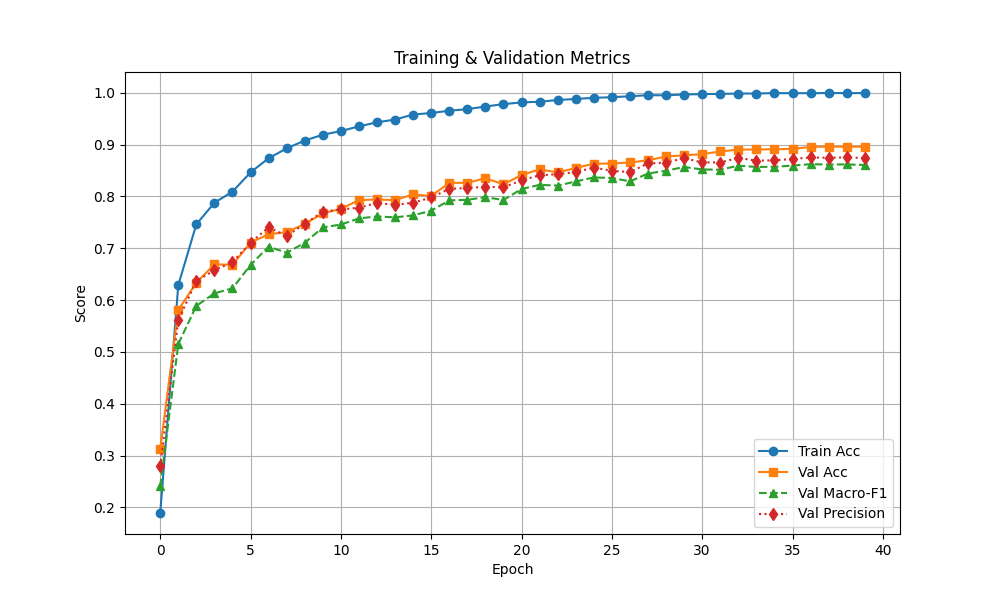
\includegraphics[width=\linewidth]{vit_b16_metrics.png}
    \caption{ViT-B/16}
\end{subfigure}
\hfill
\begin{subfigure}[b]{0.48\linewidth}
    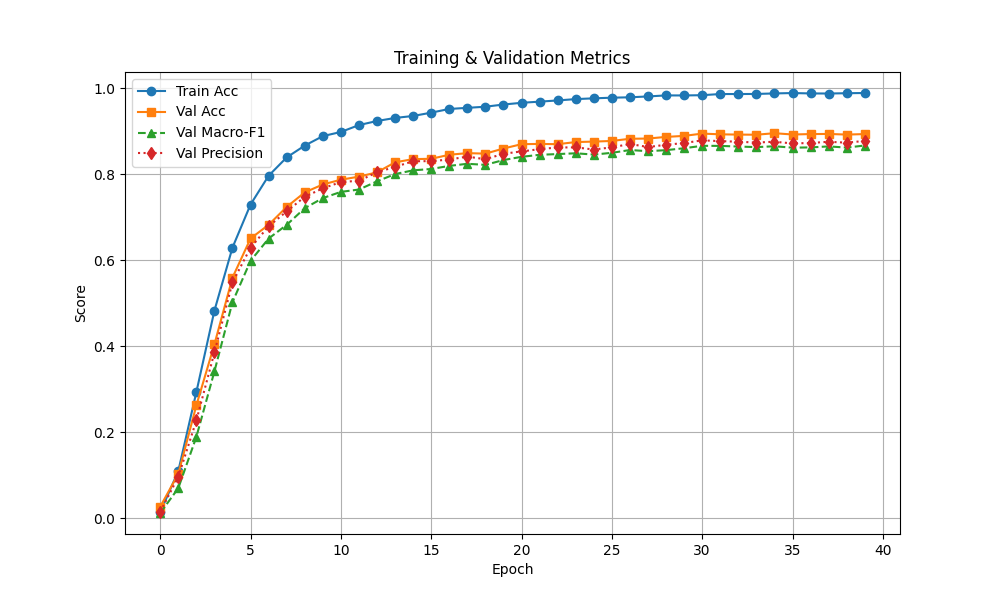
\includegraphics[width=\linewidth]{geotemporal_metrics.png}
    \caption{Geotemporal (Ours)}
\end{subfigure}
\caption{Validation metrics over 40 epochs for the two top-performing models.}
\label{fig:train_top_models}
\end{figure}

Figure~\ref{fig:train_geo_ablation} directly compares the geotemporal model against its geo-shuffled control, isolating the contribution of biogeographic priors. The genuine geotemporal signal produces consistently lower loss and higher accuracy from epoch~10 onward.

\begin{figure}[H]
\centering
\begin{subfigure}[b]{0.48\linewidth}
    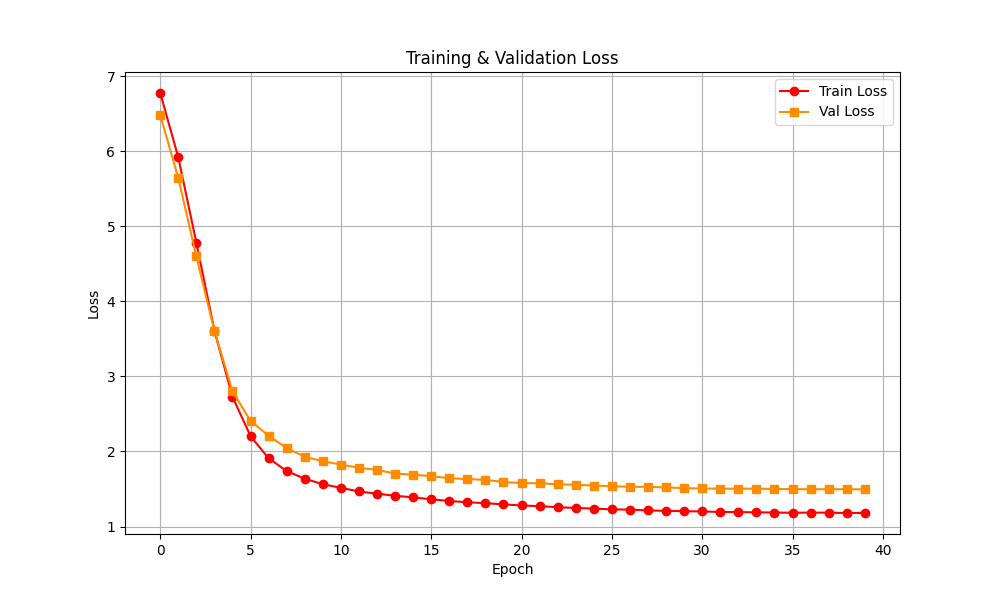
\includegraphics[width=\linewidth]{geotemporal_loss.png}
    \caption{Geotemporal -- Loss}
\end{subfigure}
\hfill
\begin{subfigure}[b]{0.48\linewidth}
    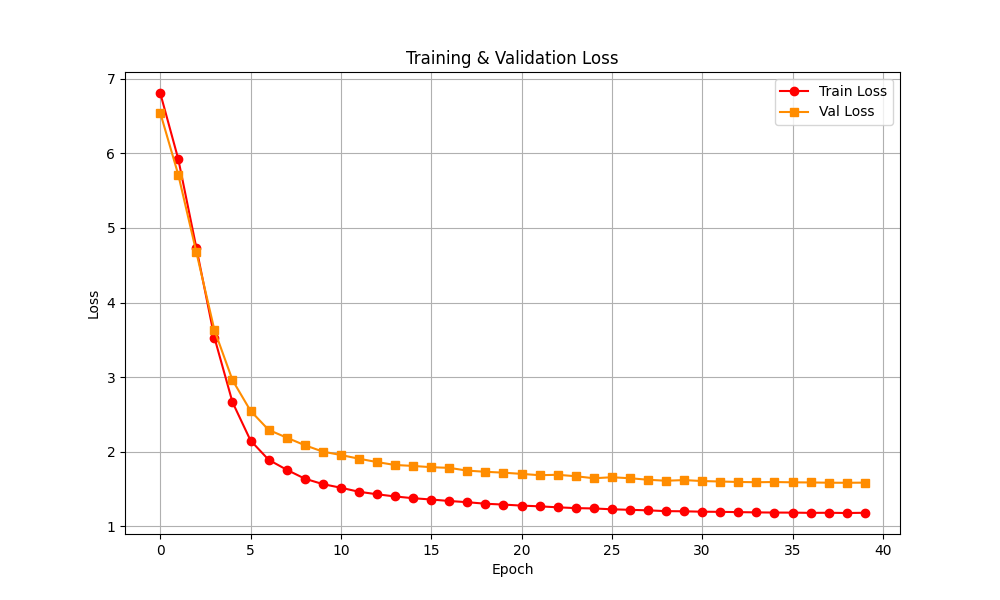
\includegraphics[width=\linewidth]{geo_shuffled_loss.png}
    \caption{Geo-Shuffled -- Loss}
\end{subfigure}
\caption{Training and validation loss: Geotemporal (left) vs Geo-Shuffled control (right). The genuine geotemporal model achieves lower final validation loss, confirming learned biogeographic priors.}
\label{fig:train_geo_ablation}
\end{figure}

Figure~\ref{fig:train_baselines} shows the training dynamics for the remaining baselines. ResNet-101 plateaus early at a low accuracy, confirming insufficient representational capacity. EfficientNet-B5 and MLFI Warmup converge to similar accuracy ranges but with different loss landscapes.

\begin{figure}[H]
\centering
\begin{subfigure}[b]{0.32\linewidth}
    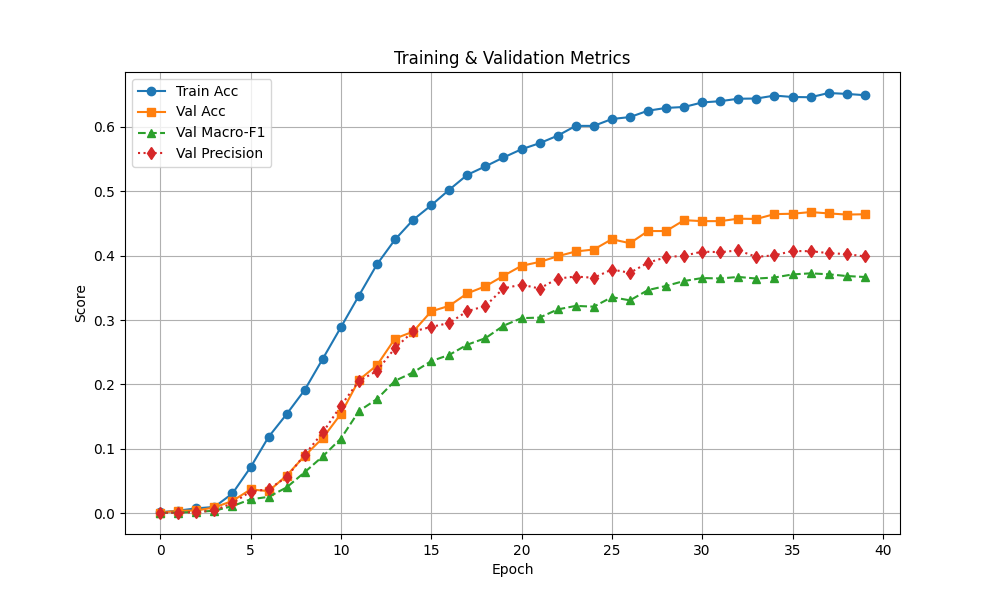
\includegraphics[width=\linewidth]{resnet101_metrics.png}
    \caption{ResNet-101}
\end{subfigure}
\hfill
\begin{subfigure}[b]{0.32\linewidth}
    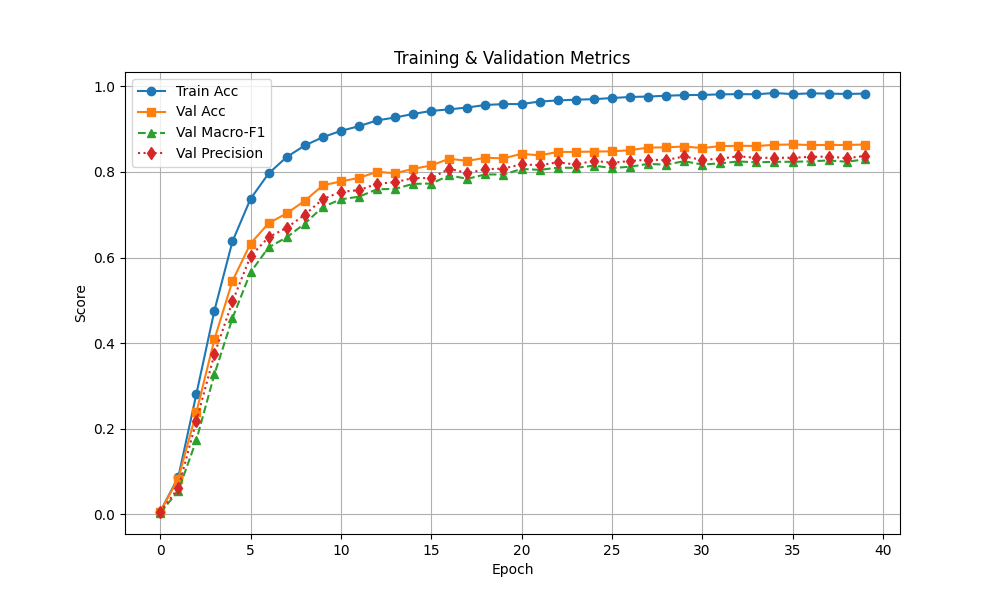
\includegraphics[width=\linewidth]{effnet_b5_metrics.png}
    \caption{EfficientNet-B5}
\end{subfigure}
\hfill
\begin{subfigure}[b]{0.32\linewidth}
    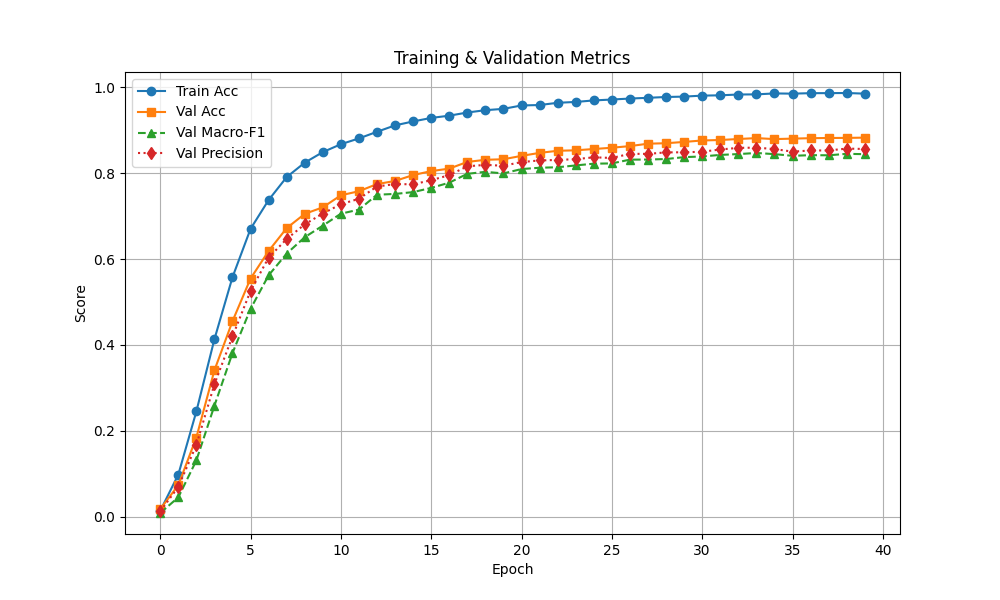
\includegraphics[width=\linewidth]{mlfi_warmup_metrics.png}
    \caption{MLFI Warmup}
\end{subfigure}
\caption{Validation metrics for baseline architectures over 40 epochs.}
\label{fig:train_baselines}
\end{figure}

\subsection{Per-Stratum Analysis}

\begin{table}[H]
\centering
\caption{Dense ($\geq$50 samples) vs Sparse ($<$50 samples) performance across models.}
\label{tab:stratum_comparison}
\small
\begin{tabular}{@{}lccccc@{}}
\toprule
\textbf{Model} & \textbf{Dense Acc} & \textbf{Dense F1} & \textbf{Sparse Acc} & \textbf{Sparse F1} & $\Delta$ \textbf{Acc (S$-$D)} \\
\midrule
ResNet-101 & 45.02 & 22.53 & 56.29 & 45.80 & +11.27 \\
EfficientNet-B5 & 87.33 & 68.30 & 86.20 & 75.07 & $-$1.13 \\
ViT-B/16 & \textbf{91.60} & \textbf{79.40} & 86.76 & 75.18 & $-$4.84 \\
MLFI Warmup & 88.36 & 73.07 & 84.86 & 72.84 & $-$3.50 \\
Geo-Shuffled & 87.87 & 72.32 & 83.32 & 71.89 & $-$4.55 \\
\textbf{Geotemporal} & 90.35 & 76.74 & \textbf{87.43} & \textbf{75.38} & $-$2.92 \\
\bottomrule
\end{tabular}
\end{table}

\subsection{Confusion Analysis}

Figure~\ref{fig:confusion_top} shows confusion matrix heatmaps for the two best-performing models. Both ViT-B/16 and our geotemporal model produce strongly diagonal matrices across 966 classes, with residual confusion concentrated in congeneric species clusters.

\begin{figure}[H]
\centering
\begin{subfigure}[b]{0.48\linewidth}
    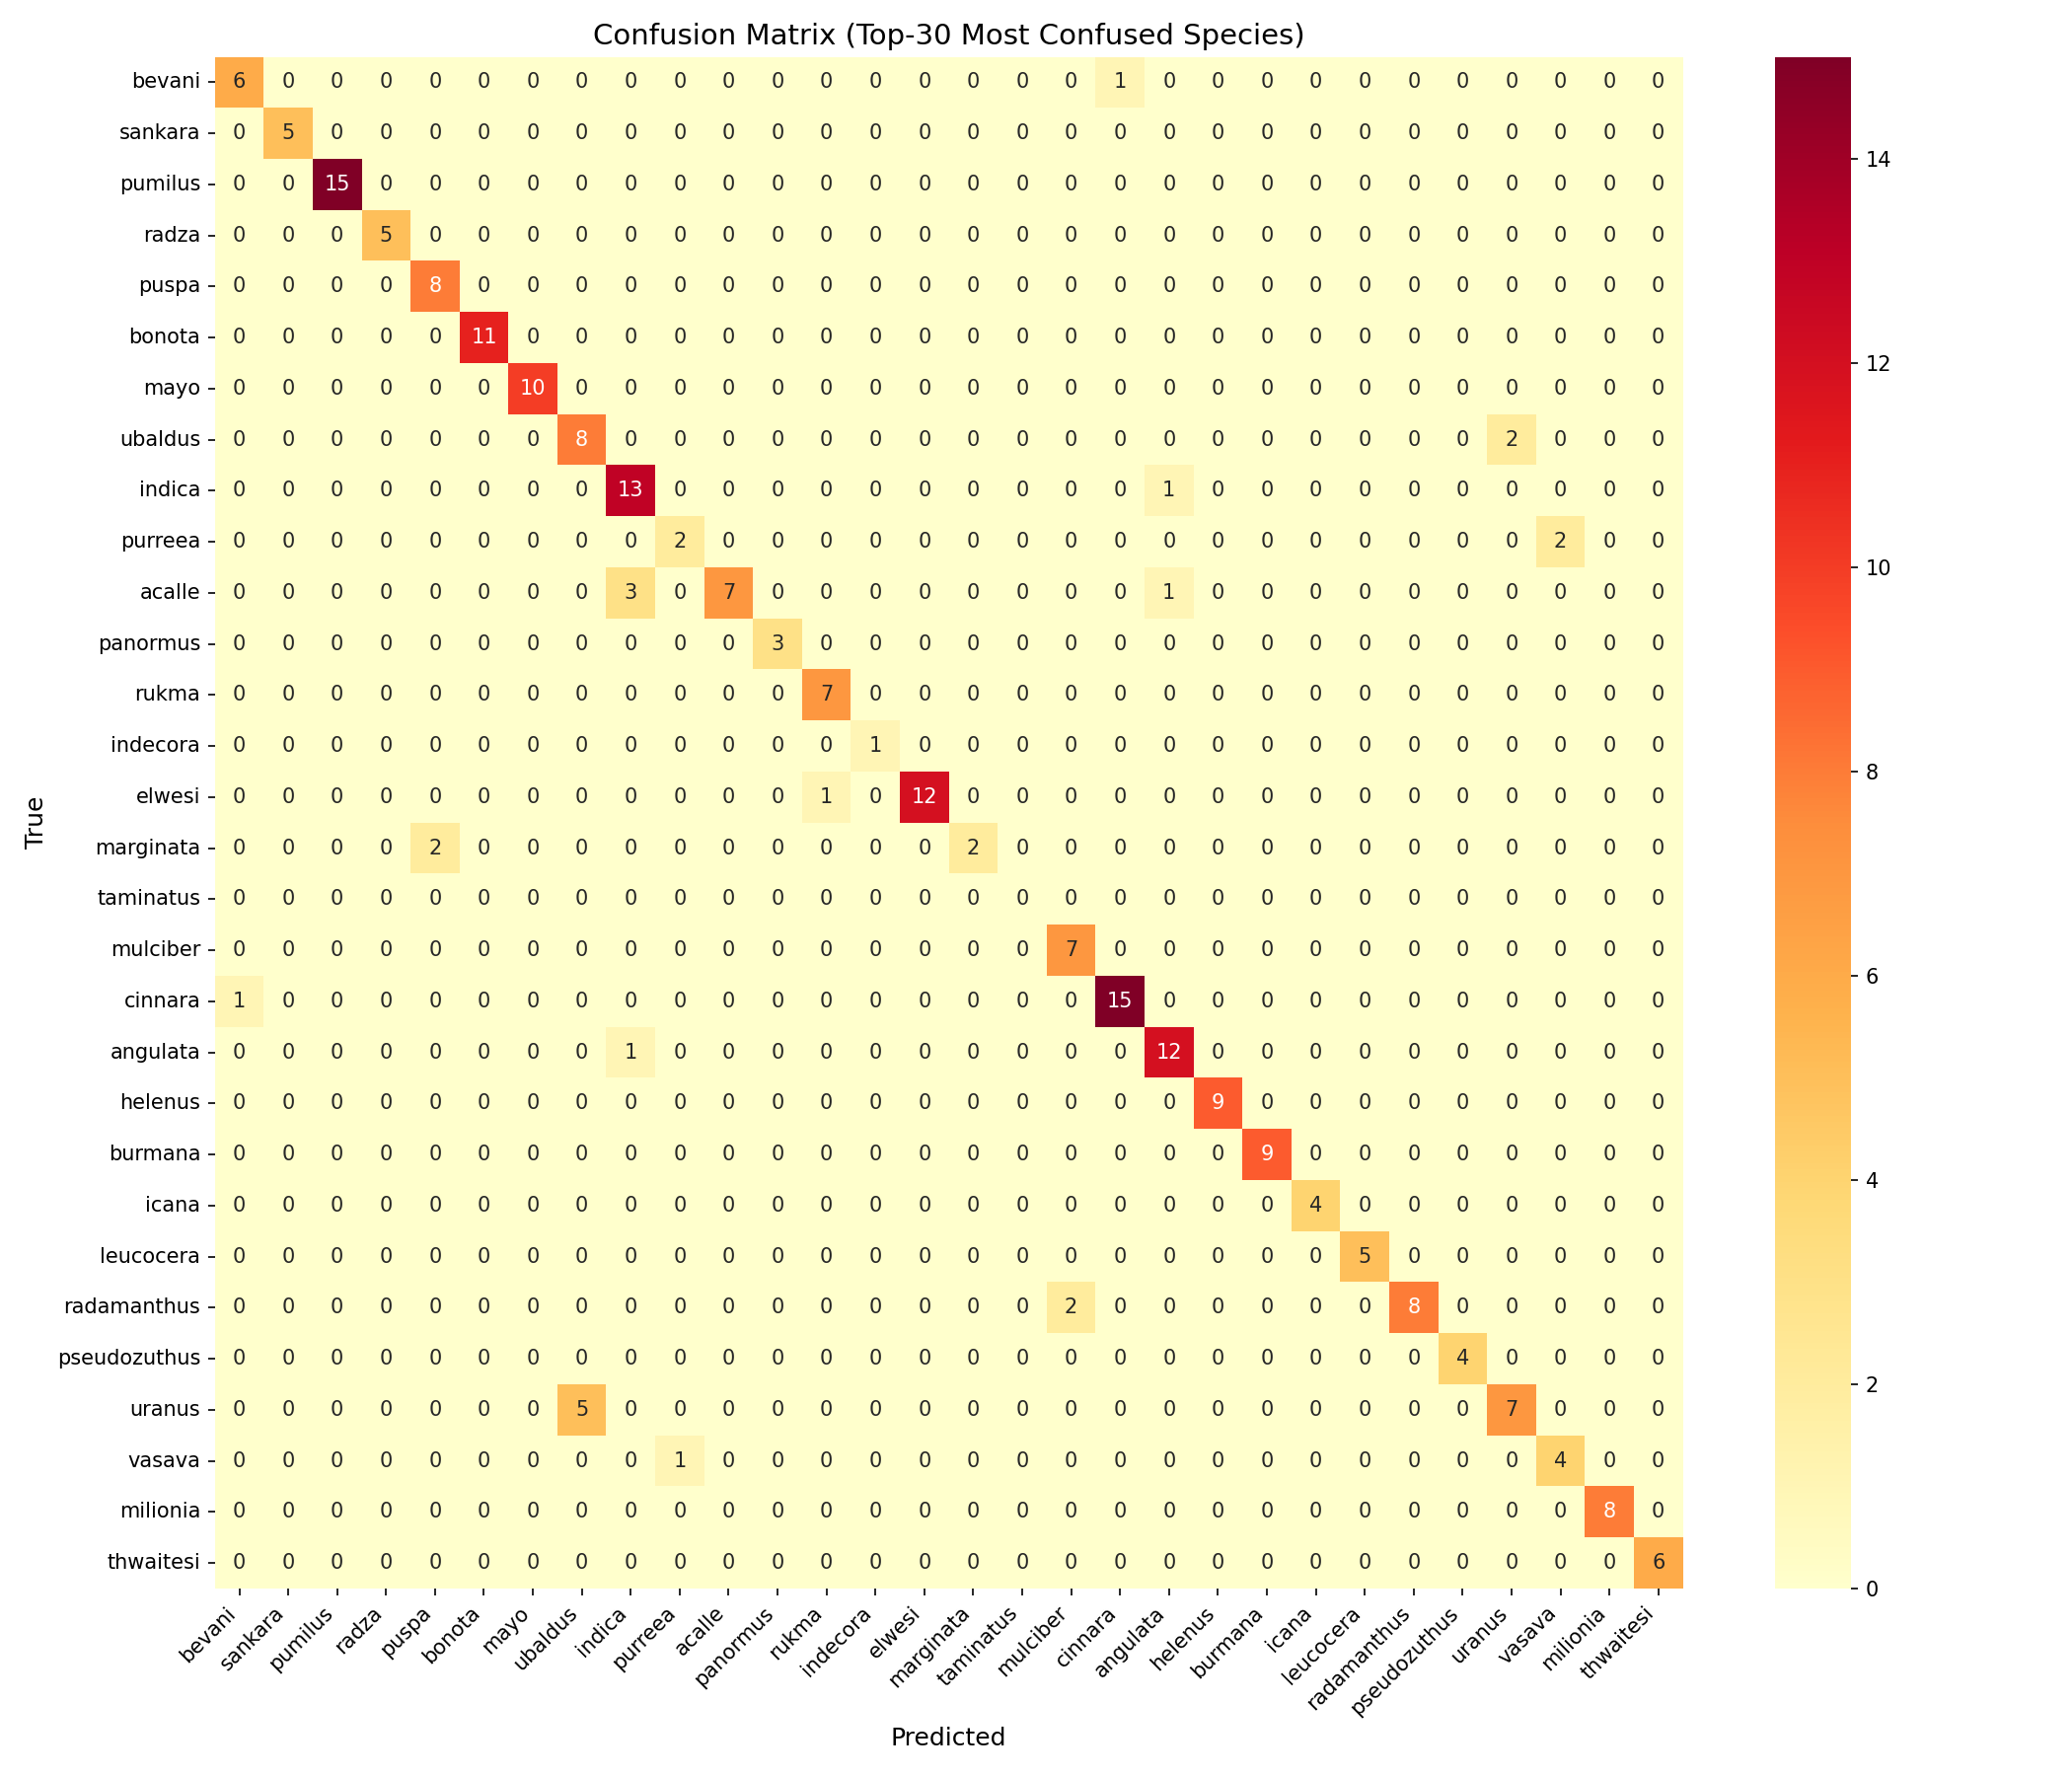
\includegraphics[width=\linewidth]{vit_b16_confusion.png}
    \caption{ViT-B/16 (89.99\% Top-1)}
\end{subfigure}
\hfill
\begin{subfigure}[b]{0.48\linewidth}
    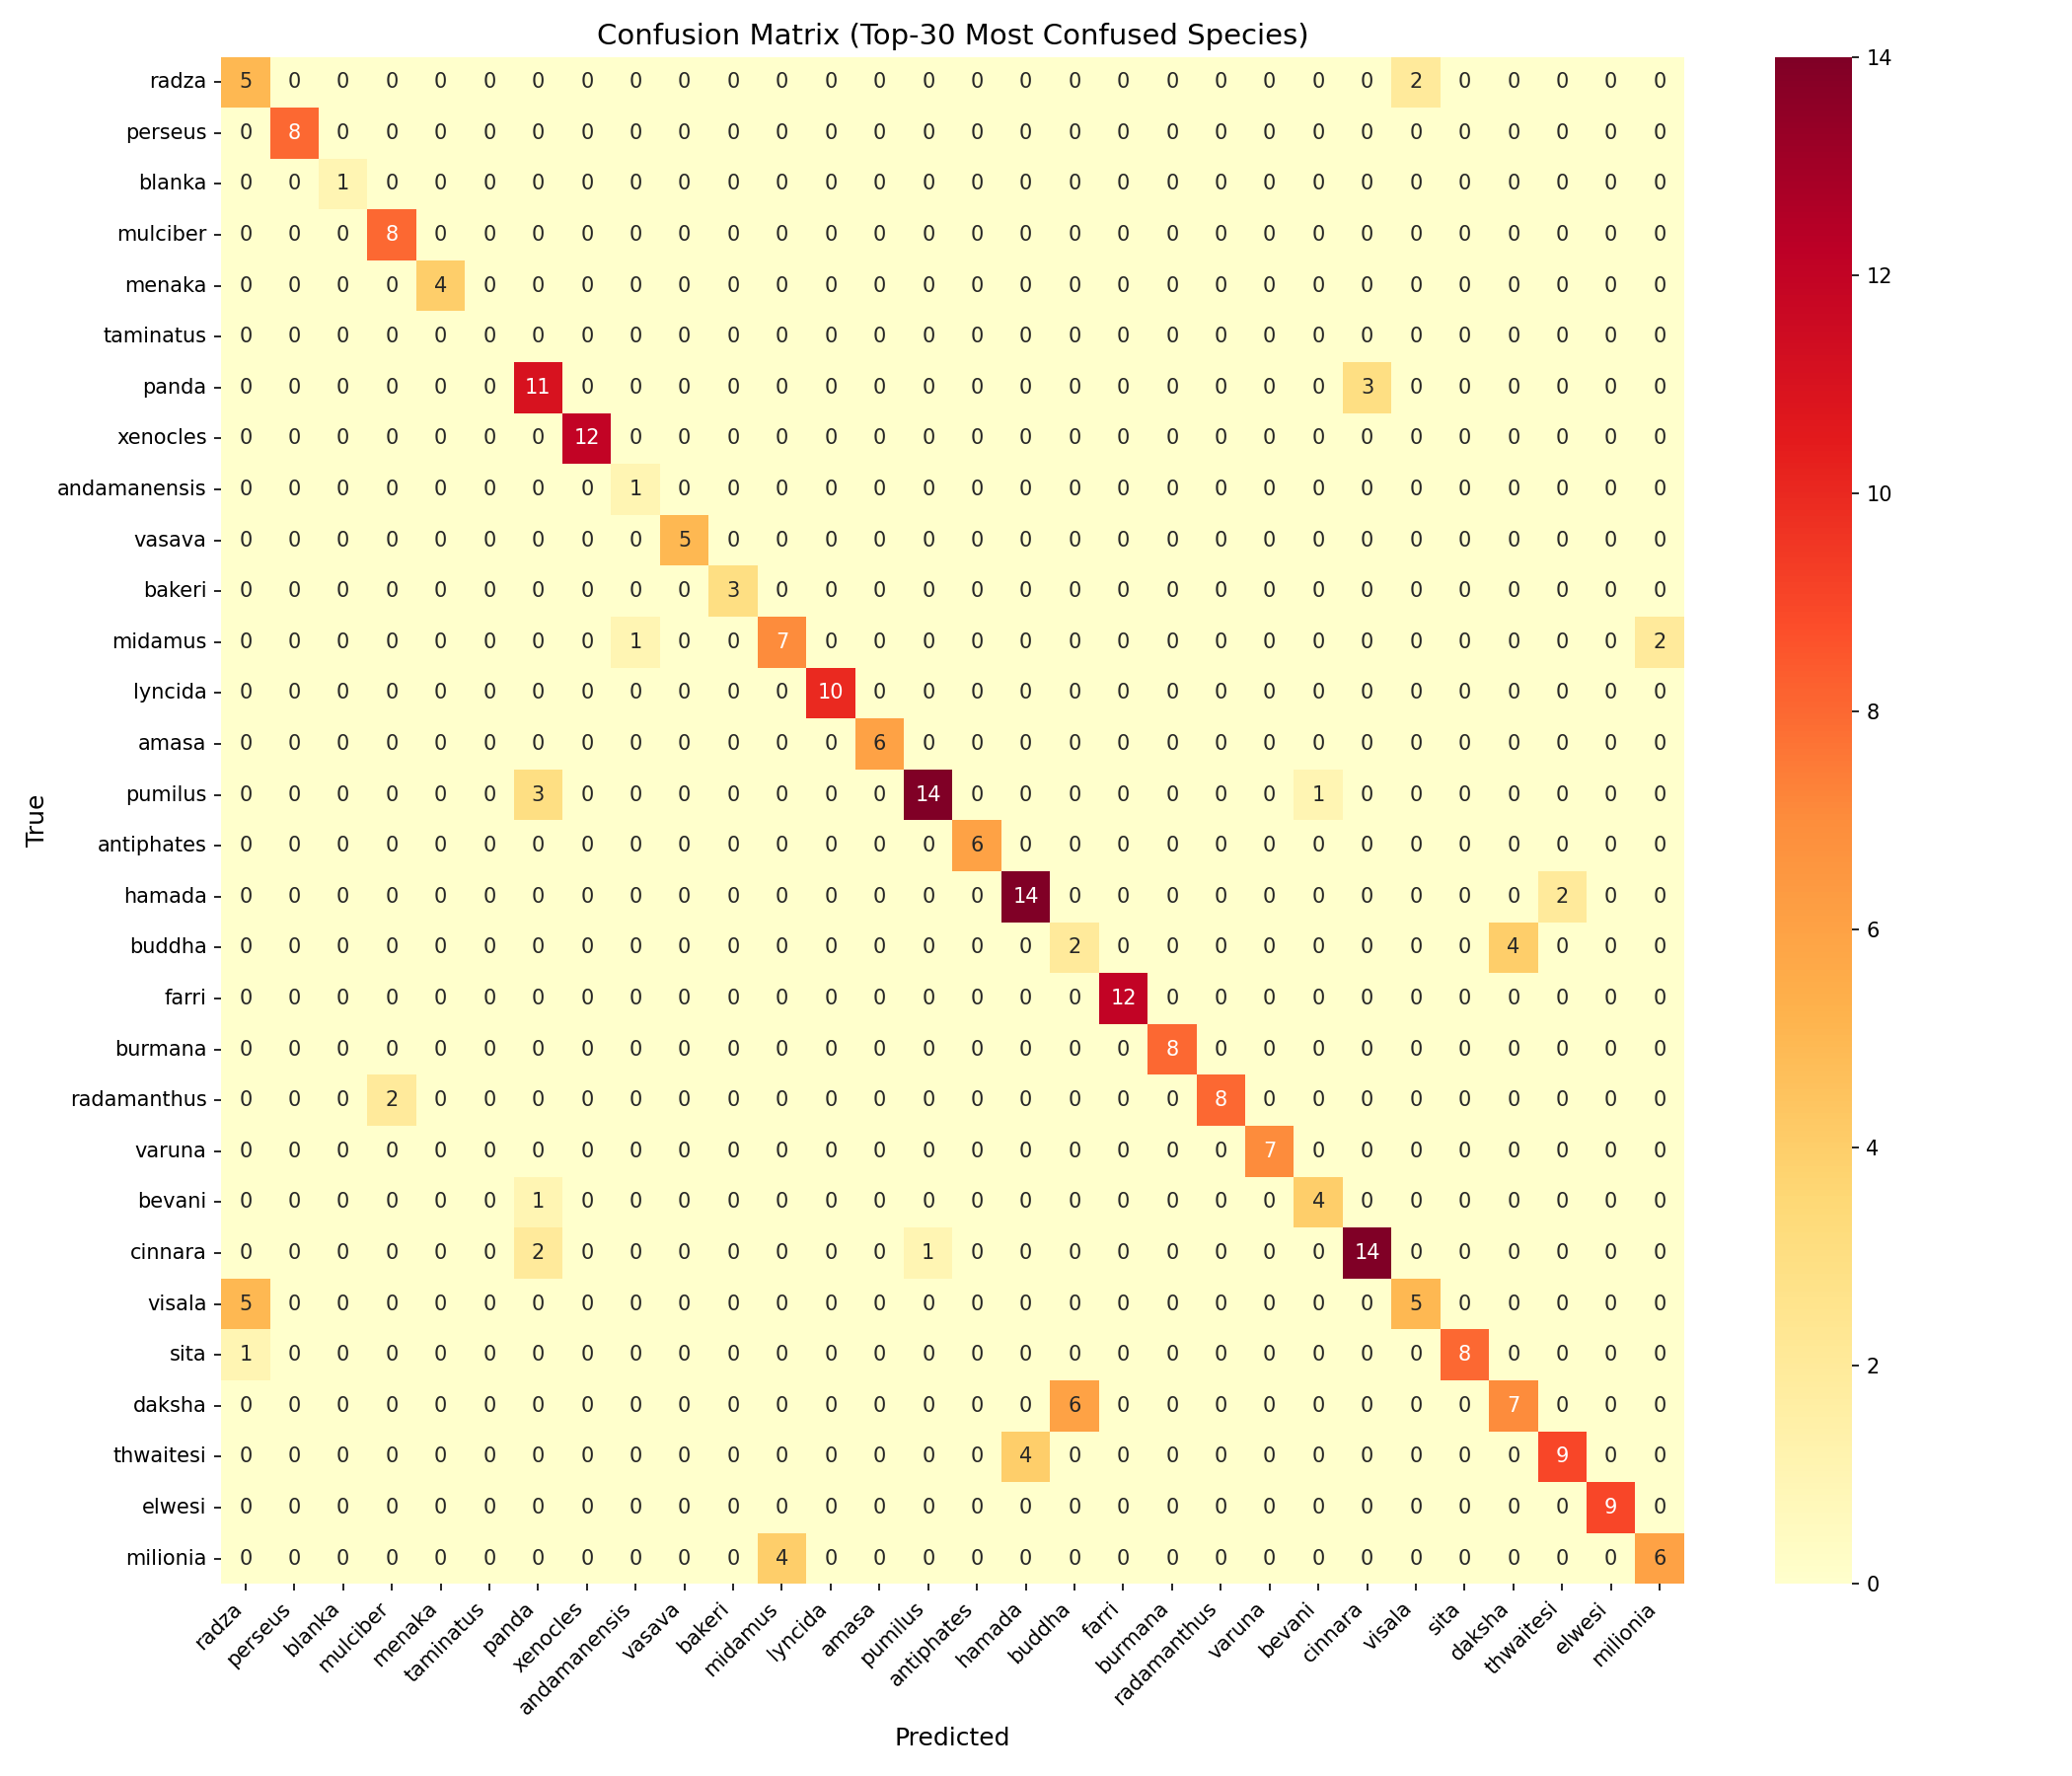
\includegraphics[width=\linewidth]{geotemporal_confusion.png}
    \caption{Geotemporal (89.38\% Top-1)}
\end{subfigure}
\caption{Confusion matrices for the two top-performing models on the 966-class test set.}
\label{fig:confusion_top}
\end{figure}

\begin{figure}[H]
\centering
\begin{subfigure}[b]{0.48\linewidth}
    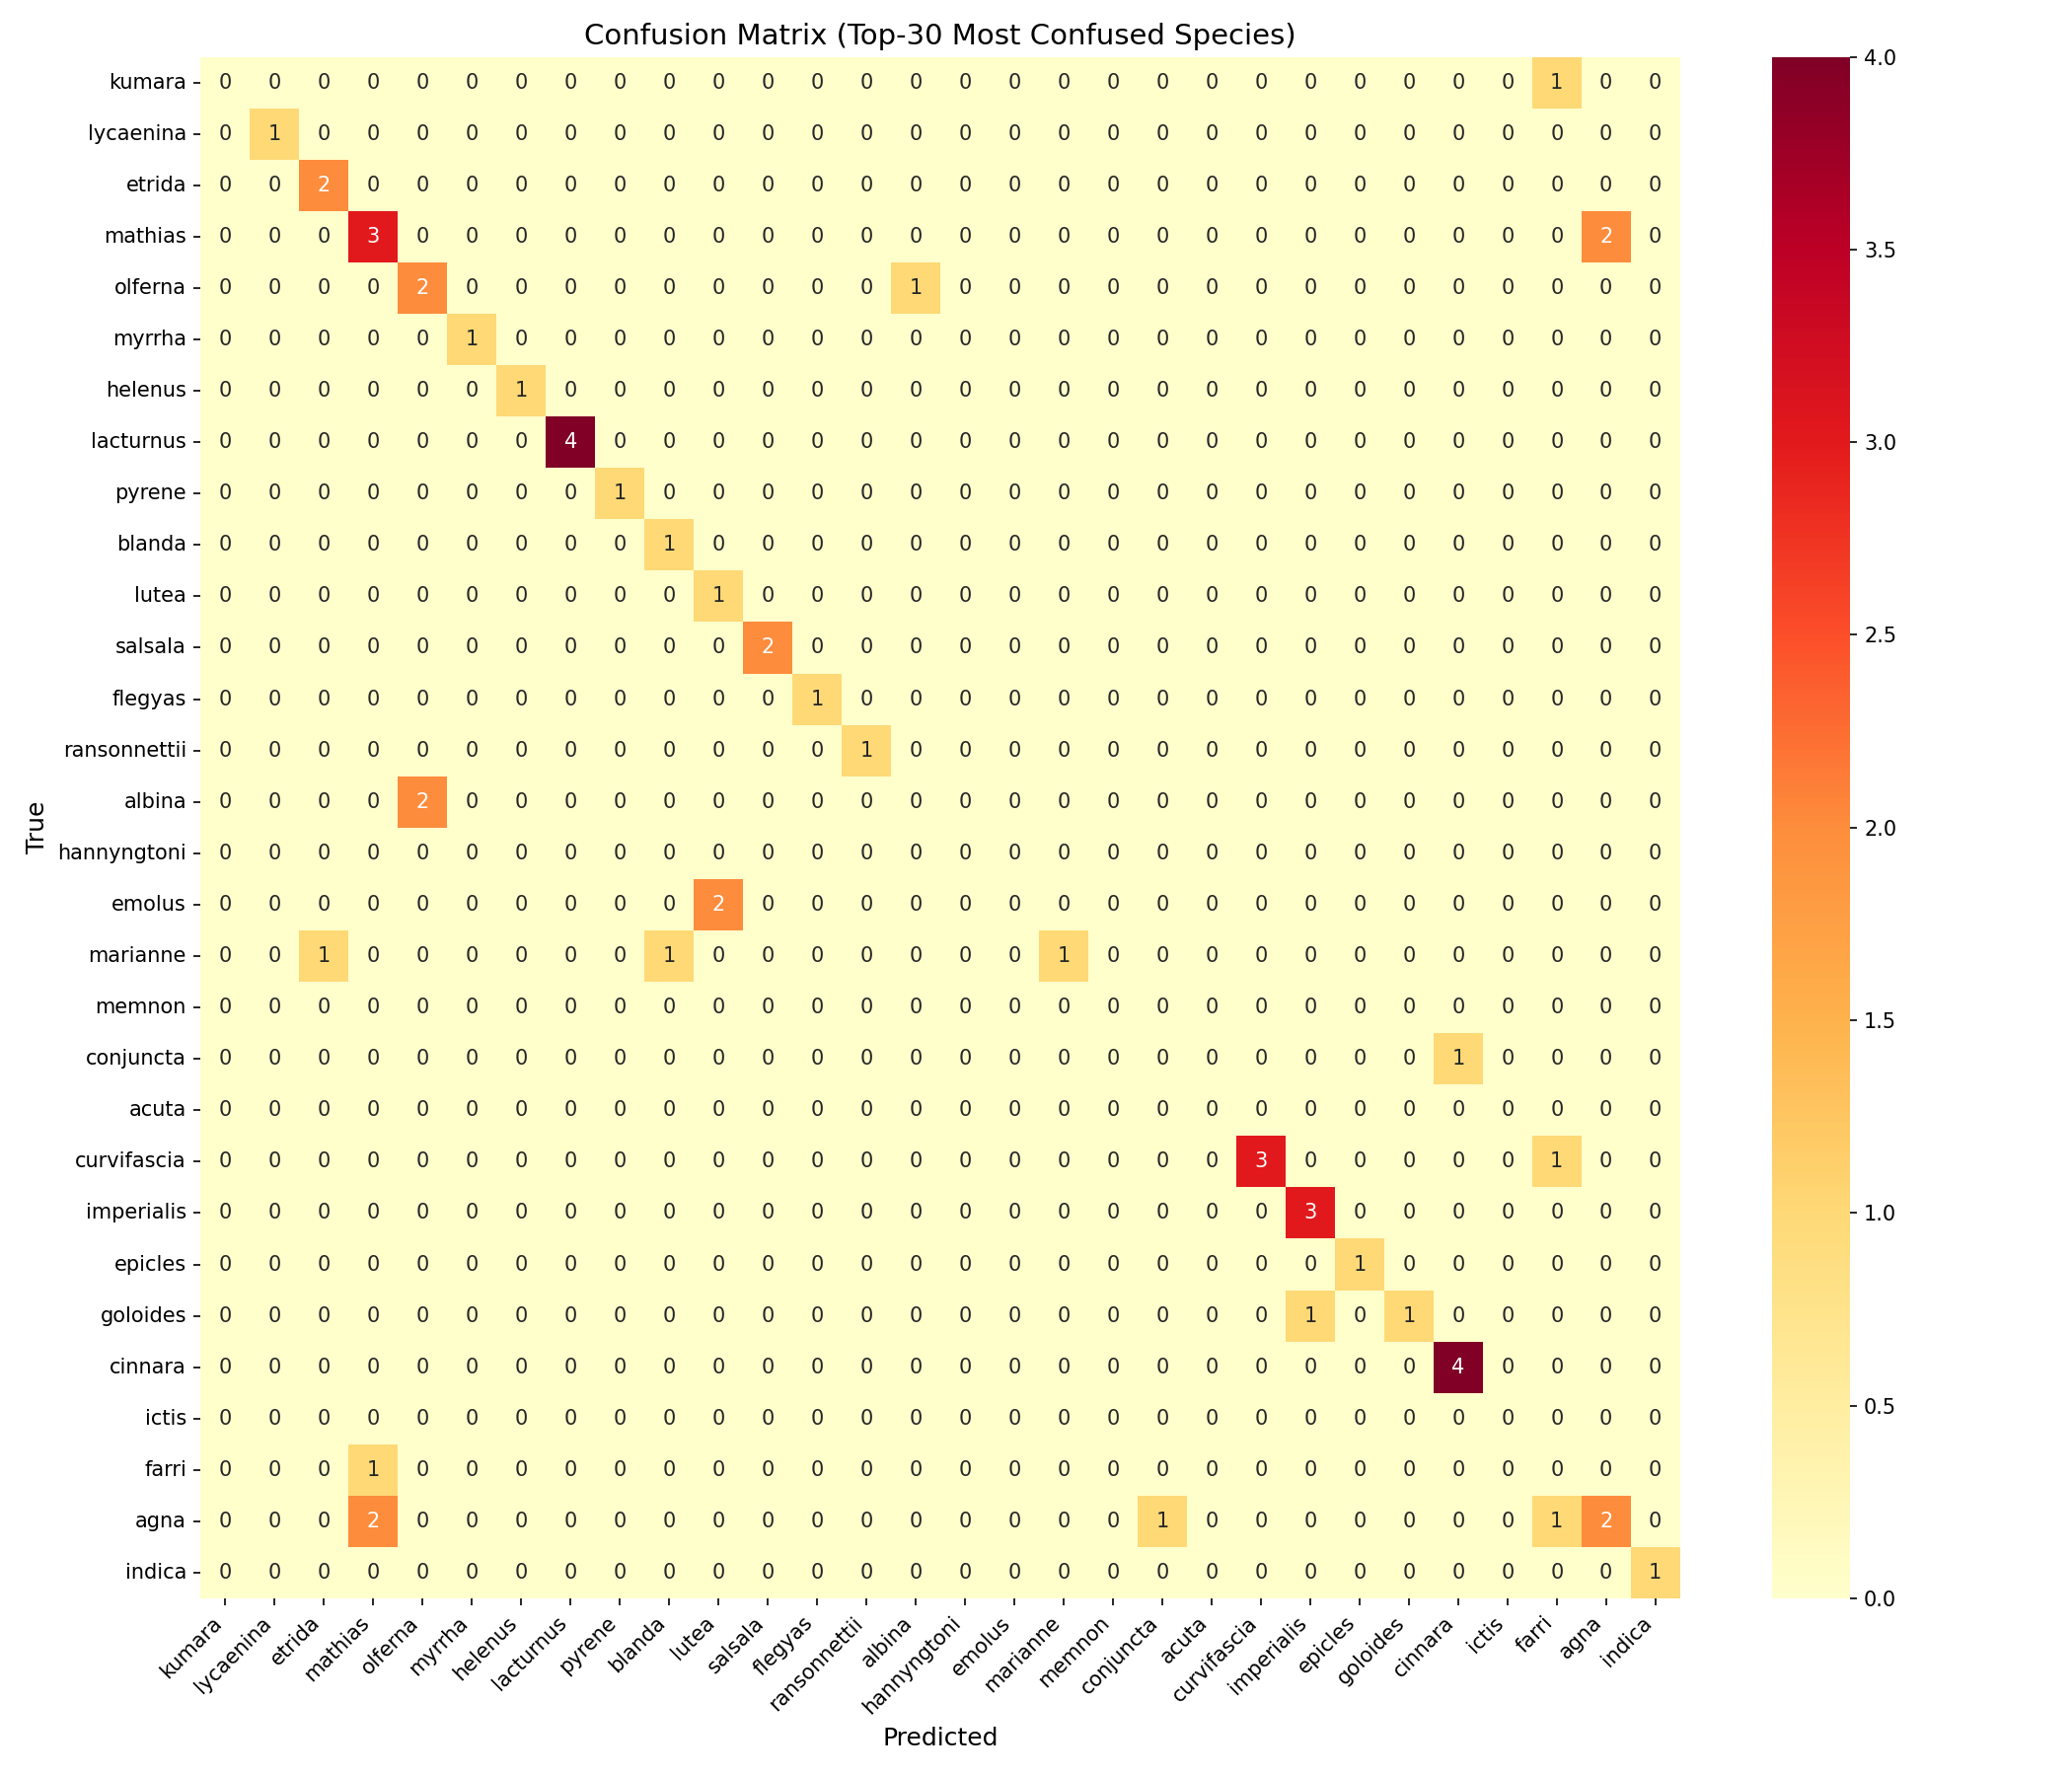
\includegraphics[width=\linewidth]{resnet101_confusion.png}
    \caption{ResNet-101 (48.76\% Top-1)}
\end{subfigure}
\hfill
\begin{subfigure}[b]{0.48\linewidth}
    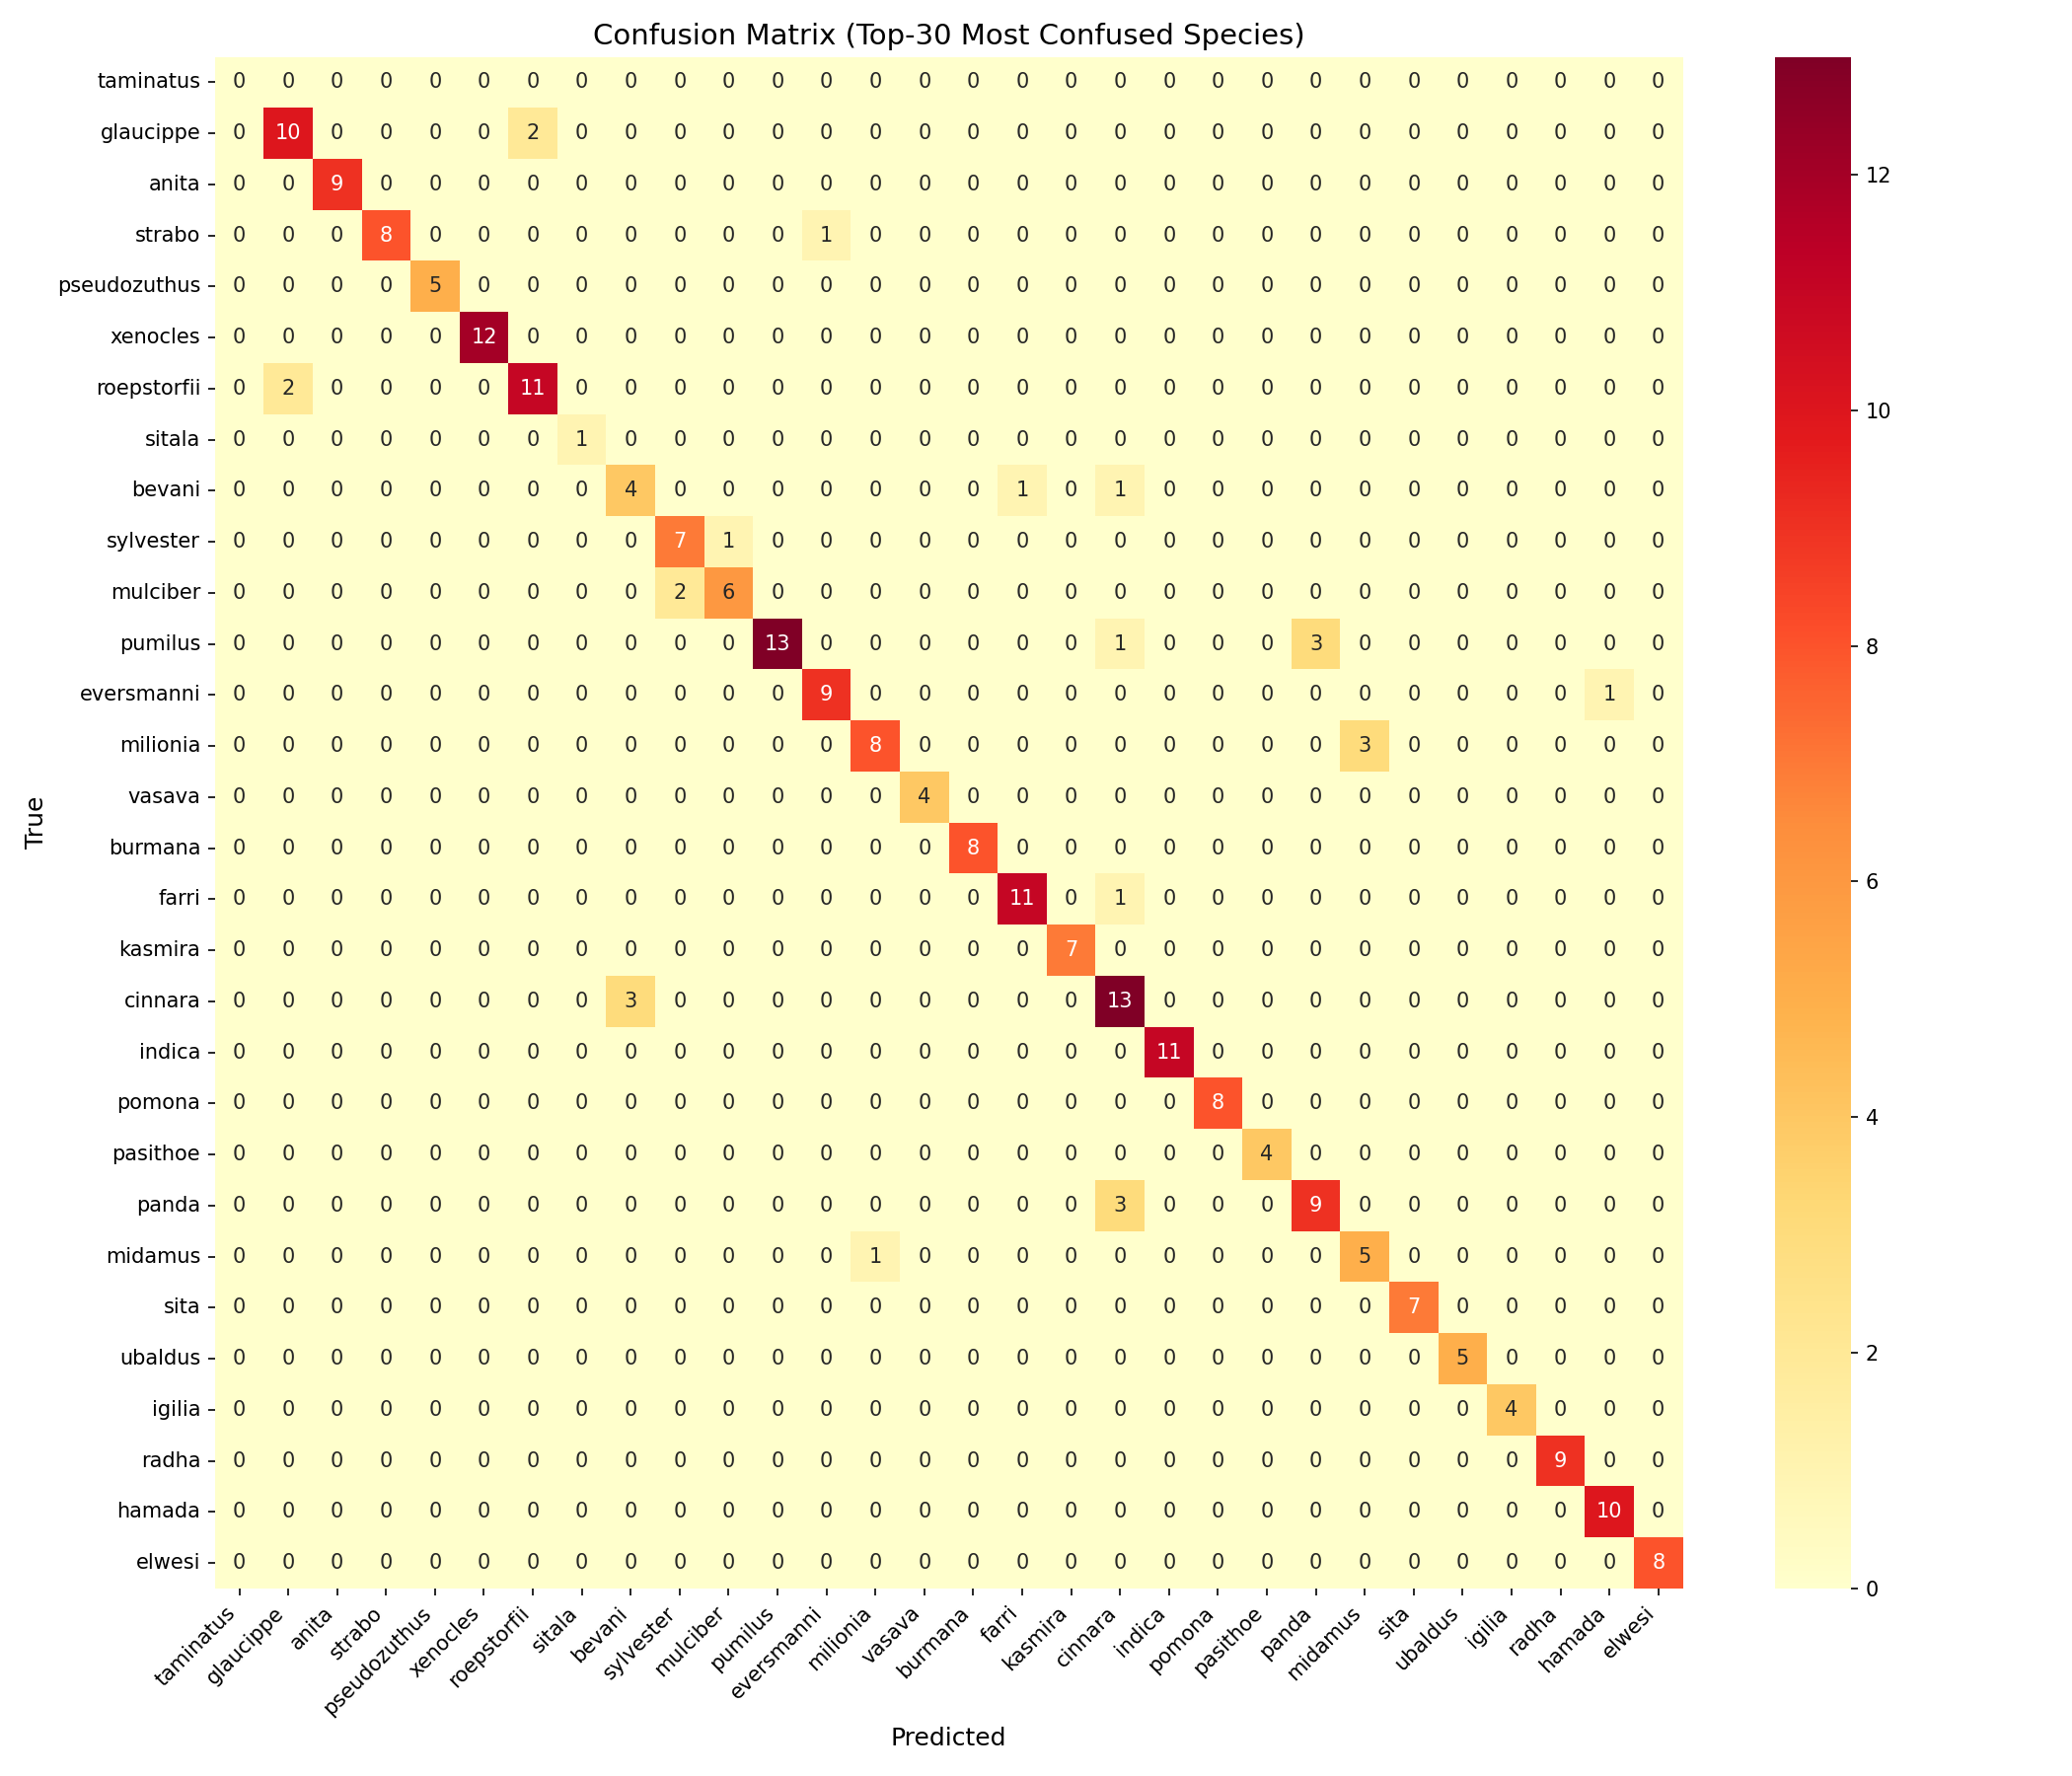
\includegraphics[width=\linewidth]{effnet_b5_confusion.png}
    \caption{EfficientNet-B5 (86.96\% Top-1)}
\end{subfigure}
\caption{Confusion matrices for baseline architectures. ResNet-101 shows diffuse off-diagonal errors across the full class space, while EfficientNet-B5 produces a near-diagonal pattern with errors concentrated in congeneric pairs.}
\label{fig:confusion_baselines}
\end{figure}

Table~\ref{tab:top_confused} lists the most-confused species pairs across models. Persistent confusion occurs between congeneric species (e.g., \emph{Papilio daksha}$\leftrightarrow$\emph{P.~buddha}, \emph{Mycalesis visala}$\leftrightarrow$\emph{M.~radza}) that share wing morphology but differ in geographic range. Our geotemporal model reduces several of these errors compared to ViT-B/16.

\begin{table}[H]
\centering
\caption{Top confused species pairs by model (test set misclassification count).}
\label{tab:top_confused}
\small
\begin{tabular}{@{}lllc@{}}
\toprule
\textbf{Model} & \textbf{True Species} & \textbf{Predicted As} & \textbf{Count} \\
\midrule
\multirow{3}{*}{ResNet-101}
  & \emph{Symbrenthia brabira} & \emph{S.~lilaea} & 7 \\
  & \emph{Eurema blanda} & \emph{E.~hecabe} & 7 \\
  & \emph{Pieris brassicae} & \emph{P.~canidia} & 5 \\
\midrule
\multirow{3}{*}{EfficientNet-B5}
  & \emph{Azanus ubaldus} & \emph{A.~uranus} & 6 \\
  & \emph{Tarucus indica} & \emph{T.~nara} & 5 \\
  & \emph{Papilio daksha} & \emph{P.~buddha} & 4 \\
\midrule
\multirow{3}{*}{ViT-B/16}
  & \emph{Tapena thwaitesi} & \emph{Taraka hamada} & 8 \\
  & \emph{Azanus uranus} & \emph{A.~ubaldus} & 5 \\
  & \emph{Papilio daksha} & \emph{P.~buddha} & 3 \\
\midrule
\multirow{3}{*}{Geotemporal}
  & \emph{Papilio daksha} & \emph{P.~buddha} & 6 \\
  & \emph{Mycalesis visala} & \emph{M.~radza} & 5 \\
  & \emph{Rapala varuna} & \emph{Remelana jangala} & 4 \\
\bottomrule
\end{tabular}
\end{table}

\subsection{Key Findings from Model Comparison}

\textbf{Geotemporal fusion is competitive with ViT-B/16.} Our geotemporal model (ConvNeXt-S + CA + MLFI + Geo, 40.8M params) achieves 89.38\% Top-1 and 88.94\% weighted F1--within 0.61 points of ViT-B/16 (86.5M params, 89.51\% weighted F1) while using 2.1$\times$ fewer parameters. It achieves the best Top-5 accuracy (98.01\%) across all models.

\textbf{Geotemporal metadata provides a genuine signal.} The geo-shuffled control (same architecture, randomized location/month) drops by $-$3.02\% Top-1 (89.38 $\to$ 86.36) and $-$2.80\% Macro-F1 (87.37 $\to$ 84.57). The training curves (Figure~\ref{fig:train_geo_ablation}) show this divergence emerges after epoch~10, confirming the geotemporal branch learns meaningful biogeographic priors rather than simply adding parameters.

\textbf{Best sparse-class performance from geotemporal model.} Our model achieves 87.43\% accuracy on sparse classes ($<$50 training images), outperforming all baselines including ViT-B/16 (86.76\%). The Dense--Sparse gap narrows to $\Delta = -2.92$ vs ViT-B/16's $\Delta = -4.84$, suggesting geotemporal priors help disambiguate underrepresented species.

\textbf{ResNet-101 confirms architectural requirements.} ResNet-101 achieves only 48.76\% Top-1 with a diffuse confusion matrix (Figure~\ref{fig:confusion_baselines}a), confirming that modern architectures with stronger inductive biases or attention mechanisms are essential for 966-class fine-grained recognition.

\textbf{Persistent congeneric confusion.} Across all models, the most-confused pairs (Table~\ref{tab:top_confused}) are congeneric species sharing wing morphology (\emph{Papilio daksha}$\leftrightarrow$\emph{P.~buddha}, \emph{Mycalesis visala}$\leftrightarrow$\emph{M.~radza}). These species have overlapping wing patterns but distinct geographic ranges and flight seasons--precisely the information encoded by geotemporal embeddings, explaining the model's advantage on sparse classes.

\section{Discussion}

Three structural constraints drive the failure modes observed across our ablation:
\begin{enumerate}[label=(\arabic*)]
    \item \textbf{Spatial collapse} in standard attention mechanisms obscures the precise localisation needed for wing pattern discrimination. Coordinate Attention addresses this by preserving directional spatial maps, yielding the highest Sparse-class accuracy (88.05\%) in the ablation study.
    \item \textbf{Progressive texture loss} through repeated pooling destroys fine-grained cues essential for species differentiation. MLFI addresses this through early-layer feature preservation, achieving strong Sparse performance (86.66\%), but the added parameterisation creates optimisation difficulties that limit overall accuracy.
    \item \textbf{Class imbalance} under uniform sampling starves rare species of gradient signal. Balanced CE sampling achieves the highest macro-F1 (85.48\%) by compressing the Dense--Sparse accuracy gap to 1.83 points.
\end{enumerate}

The domain-shift finding is the most generalisable insight. The Head-Only configuration's 53.20\% accuracy--with Dense-class accuracy (44.46\%) falling below Sparse-class accuracy (70.75\%)--demonstrates that ImageNet features are not merely insufficient but structurally inappropriate for entomological morphology.

The model comparison study extends these findings: geotemporal fusion effectively bridges the remaining accuracy gap by providing ecological context that the visual features alone cannot capture. The most confused species pairs (e.g., \emph{Papilio daksha}$\leftrightarrow$\emph{P.~buddha}, \emph{Mycalesis visala}$\leftrightarrow$\emph{M.~radza}) are congeneric species with overlapping wing patterns but distinct geographic ranges and flight seasons--precisely the signal that geotemporal embeddings encode.

These findings extend beyond butterflies to medical imaging, satellite-based crop monitoring, and microscopy-based cell classification--all domains facing similar constraints of extreme class imbalance, domain-specific morphological features, and limited per-class training data~\cite{amarathunga2022thrips}.

\section{Conclusion}

Four key findings emerge from our comprehensive evaluation:
\begin{enumerate}[label=(\arabic*)]
    \item \textbf{Geotemporal fusion matches ViT-B/16 at half the parameters:} Our ConvNeXt-S + CA + MLFI + Geo model (40.8M params) achieves 89.38\% Top-1 and the best Top-5 (98.01\%), within 0.61 points of ViT-B/16 (86.5M params). Geo-shuffled ablation confirms this is genuine biogeographic signal ($-$3.02\% on permutation).
    \item \textbf{Balanced sampling dominates:} CE + Balanced achieves the best ablation macro-F1 (85.48\%) with the most equitable stratum performance. Focal Loss improves Sparse-class accuracy but at the cost of Dense-class performance.
    \item \textbf{Coordinate Attention is high-value, low-cost:} CA adds minimal parameters yet improves Sparse-class accuracy by 1.29 points (88.05\%), making it the optimal architectural intervention.
    \item \textbf{ImageNet transfer fails catastrophically:} Head-Only achieves 53.20\%--full end-to-end fine-tuning is mandatory for specialised biological domains.
\end{enumerate}

Future work includes prototypical network heads~\cite{snell2017prototypical} for the $\sim$627 classes with $<$50 images, domain-specific self-supervised pretraining (DINO on butterfly images)~\cite{feichtenhofer2022masked} to bootstrap features from unlabelled in-domain data, and integration of host-plant association features for habitat-aware species prediction.

\newpage

\bibliographystyle{plainnat}

\begin{thebibliography}{15}

\bibitem[Yuan et~al., 2025]{yuan2025fgbnet}
Y.~Yuan et~al., FGBNet: A Bio-Subspecies Classification Network with Multi-Level Feature Interaction, \emph{Diversity}, 2025. \url{https://doi.org/10.3390/d17040237}

\bibitem[Hou et~al., 2021]{hou2021coordinate}
Q.~Hou, D.~Zhou, and J.~Feng, Coordinate Attention for Efficient Mobile Network Design, \emph{CVPR}, 2021. \url{https://arxiv.org/abs/2103.02907}

\bibitem[Liu et~al., 2022]{liu2022convnext}
Z.~Liu, H.~Mao, C.-Y.~Wu, C.~Feichtenholer, T.~Darrell, and S.~Xie, A ConvNet for the 2020s, \emph{CVPR}, 2022. \url{https://arxiv.org/abs/2201.03545}

\bibitem[Hu et~al., 2018]{hu2018squeeze}
J.~Hu, L.~Shen, and G.~Sun, Squeeze-and-Excitation Networks, \emph{CVPR}, 2018. \url{https://arxiv.org/abs/1709.01507}

\bibitem[Lin et~al., 2017]{lin2017focal}
T.-Y.~Lin, P.~Goyal, R.~Girshick, K.~He, and P.~Doll\'{a}r, Focal Loss for Dense Object Detection, \emph{ICCV}, 2017. \url{https://arxiv.org/abs/1708.02002}

\bibitem[Amarathunga et~al., 2022]{amarathunga2022thrips}
D.~C.~Amarathunga et~al., Fine-grained image classification of microscopic insect pest species, \emph{Computers and Electronics in Agriculture}, 2022. \url{https://doi.org/10.1016/j.compag.2022.107462}

\bibitem[Snell et~al., 2017]{snell2017prototypical}
J.~Snell, K.~Swersky, and R.~Zemel, Prototypical Networks for Few-Shot Learning, \emph{NeurIPS}, 2017. \url{https://arxiv.org/abs/1703.05175}

\bibitem[Feichtenhofer et~al., 2022]{feichtenhofer2022masked}
C.~Feichtenhofer, H.~Fan, Y.~Li, and K.~He, Masked autoencoders as spatiotemporal learners, \emph{NeurIPS}, 2022. \url{https://proceedings.neurips.cc/paper_files/paper/2022/file/e97d1081481a4017df96b51be31001d3-Paper-Conference.pdf}

\bibitem[Dosovitskiy et~al., 2021]{dosovitski2021image}
A.~Dosovitskiy et~al., An image is worth 16x16 words: Transformers for image recognition at scale, \emph{ICLR}, 2021. \url{https://arxiv.org/pdf/2010.11929}

\bibitem[Loshchilov and Hutter, 2017]{loshchilov2017sgdr}
I.~Loshchilov and F.~Hutter, SGDR: Stochastic Gradient Descent with Warm Restarts, \emph{ICLR}, 2017. \url{https://arxiv.org/abs/1608.03983}

\bibitem[Wah et~al., 2011]{wah2011cub}
C.~Wah, S.~Branson, P.~Welinder, P.~Perona, and S.~Belongie, The Caltech-UCSD Birds-200-2011 Dataset, Technical Report CNS-TR-2011-001, Caltech, 2011.

\bibitem[Van~Horn et~al., 2018]{vanhorn2018inaturalist}
G.~Van~Horn et~al., The iNaturalist Species Classification and Detection Dataset, \emph{CVPR}, 2018. \url{https://arxiv.org/abs/1707.06642}

\end{thebibliography}

\end{document}